\section{Data}
\label{sec:Data}
In order to enforce reproducibility of results, this section provides a detailed description of the setup used in order to generate the synthetic data utilized in the results section, as well as the real datasets.

\subsection{Synthetic Data}
\label{sec:Data:SyntheticData}
The synthetic data used for validating the Constant Velocity Model is generated in order to be in possession of a ground truth set of parameters with which the model can be evaluated.
Mathematically, the data is based int the Poisson process explained in detail under section \ref{sec:Method:Poisson}.

The ground truth parameters that need to be determined are how many nodes $N$ are in the desired system, their initial positions $Z$, their initial velocities $V$ and the $\beta$ background intensity.
One further parameter that has to be determined is the max time with which interactions are counted in, meaning interactions of time $t > t_{max}$ are not included in the synthetic dataset.


\subsubsection{Synthetic Dataset 1}
\label{sec:Data:SyntheticData:SyntheticDataset1}
The first synthetic dataset is small, consisting of four nodes, and will only be utilized in order to evaluate the Constant Velocity Model in a one-step setting.

The ground truth parameters of the first synthetic dataset are as follows:
\begin{equation}
    N = 4, \hspace{10}
    t_{max} = 10, \hspace{10}
    Z = \left( \begin{matrix}
                -0.6 & 0.0\\
                0.6 & 0.1\\
                0.0 & 0.6\\
                0.0 & -0.6
                \end{matrix}\right), \hspace{10}
    V = \left( \begin{matrix}
                0.09 & 0.01\\
                -0.01 & -0.01\\
                0.01 & -0.09\\
                -0.01 & 0.09
                \end{matrix}\right), \hspace{10}
    \beta = 7.5
\end{equation}
These ground parameters yield a dataset, tuples denoting the two interacting nodes $u$ and $v$ as well as the time of interaction $t$, ie. $(u_i, v_i, t_i)$, which has size $n=79,424$.


\subsubsection{Synthetic Dataset 2}
\label{sec:Data:SyntheticData:SyntheticDataset2}
The second synthetic dataset is utilized in order to test the modelling capabilities of the stepwise Constant Velocity Model. 

In order to generate a dataset which has attributes that make sense modelling using a stepwise approach, the velocities of the nodes is changed over the timespan from 0 to $t_{max}$.
For synthetic dataset 2, five nodes are each attributed a starting position and 10 velocity vectors.

The ground truth parameters of the second synthetic dataset are as follows:
\begin{equation}
    N = 5, \hspace{10}
    t_{max} = 50, \hspace{10}
    Z = \left( \begin{matrix}
                1 & 1\\
                1 & -1\\
                -1 & 1\\
                -1 & -1\\
                0 & 2
                \end{matrix}\right), \hspace{10}
    V_1 = \left( \begin{matrix}
                -0.15 & -0.15\\
                -0.15 & 0.15\\
                0.15 & -0.15\\
                0.15 & 0.15\\
                0.05 & -0.3
                \end{matrix}\right)... 
    V_{10} = \left( \begin{matrix}
                -0.15 & 0.05\\
                -0.15 & -0.05\\
                0.15 & -0.05\\
                0.15 & 0.05\\
                0.1 & 0.05
                \end{matrix}\right), \hspace{10}
    \beta = 7.5
\end{equation}
These ground parameters yield a dataset which has size $n=330,023$.



\subsubsection{Synthetic Dataset 3}
\label{sec:Data:SyntheticData:SyntheticDataset3}
The third synthetic dataset is utilized in order to test scalability of the model, and for this purpose it is changeable in terms of number of nodes and beta value.
The number of nodes is chosen from the following range of $N$'s:
\begin{equation}
    N = [2, 4, 6, 8, 10, 12, 14, 16, 18, 20, 22, 24, 26, 28, 30, 34, 38, 42, 46, 50, 60]
\end{equation}
For the dataset consisting of $N = 2$ nodes, the starting positions are:
\begin{equation}
        Z = \left( \begin{matrix}
                1.0 & 0.0\\
                -1.0 & 0.0\\
                \end{matrix}\right)
\end{equation}
For the dataset consisting of $N = 6$ nodes, four more nodes are added which are placed further up along the y-axis, as the following:
\begin{equation}
        Z = \left( \begin{matrix}
                1.0 & 0.0\\
                -1.0 & 0.0\\
                1.0 & 1.0\\
                -1.0 & 1.0\\
                1.0 & 2.0\\
                -1.0 & 2.0\\
                \end{matrix}\right)
\end{equation}
The beta value $\beta$ is, like the number of nodes, also chosen from a range as follows:

\begin{equation}
    \beta = [5.0, 5.25, 5.5, 5.75, 6.0, 6.25, 6.5, 6.75, 7.0, 7.25, 7.5, 7.75, 8.0, 8.25, 8.5, 8.75, 9.0]
\end{equation}
The max time is $t_{max} = 20$, and as such the remaining ground truth parameter of the third synthetic dataset is the velocities of the four steps, which are replicated for each added set of nodes:
\begin{equation}
    
    V_1 = \left( \begin{matrix}
                -0.2 & -0.05\\
                0.2 & 0.05\\
                \end{matrix}\right), \hspace{5}
    V_2 = \left( \begin{matrix}
                0.2 & 0.05\\
                -0.2 & -0.05\\
                \end{matrix}\right), \hspace{5}
    V_3 = \left( \begin{matrix}
                -0.3 & -0.05\\
                0.3 & 0.05\\
                \end{matrix}\right), \hspace{5}
    V_4 = \left( \begin{matrix}
                0.3 & 0.05\\
                -0.3 & -0.05\\
                \end{matrix}\right)
\end{equation}


\subsection{Real Data}
\label{sec:Data:RealData}


\subsubsection{Real Dataset 1: Player Interactions in a game of 'Resistance'}
\label{sec:Data:RealData:RealDataset1}
Dataset can be found here: \href{https://snap.stanford.edu/data/comm-f2f-Resistance.html}{https://snap.stanford.edu/data/comm-f2f-Resistance.html}
\\\\
The first real-life dataset consists of player interactions in a game of Resistance.

The Resistance game is a discussion, find-the-fraudster game, in which each player has a role belonging to either the resistance (good guys) or government spies (evil guys).
Only the government spies know the identity of their teammates, and so the goal of the game is for the resistance to identify the spies through verbal communication and vote them out, while the spies try to vote out the resistance by convincing their opponents of their innocence. 
The interactions they make consist in one player addressing another player verbally, and the eight most clear interactions have been recorded for each timestep, which consist in thirds of a second. 
The players can also address the computer for hints, but it cannot address the players.

The specific dataset, game 4 of the included 62 games in the dataset, has eight players and a computer, ie. nine nodes, making 58.584 interactions spanning from time $t_{min} = \frac{0}{3}$ seconds to $t_{max} = \frac{7322}{3}$ seconds, approximately $40$ minutes and $40$ seconds.

The timestamps are transformed from thirds of a second to minutes by the following formula:

\begin{equation}
    t_i = 40.67 \cdot \frac{t_i - t_{min}}{t_{max}}
\end{equation}
The overall distribution of interactions are completely uniformly distributed due to the recording process.



\subsubsection{Real Dataset 2: EU Research Institution Email Correspondences}
\label{sec:Data:RealData:RealDataset2}
Dataset can be found here: \href{https://snap.stanford.edu/data/email-Eu-core-temporal.html}{https://snap.stanford.edu/data/email-Eu-core-temporal.html}
\\\\
The second real-life dataset consists of email correspondences between institution members.
The original dataset consists of 332.334 member-interactions (email exchanges) timestamped in seconds, with the first email being sent at time $t_{min} = 0$ seconds and the last email being sent at 69.459.254 seconds, 803 days after the first.
The dataset is reduced to 329.910 interactions due to a large empty gap between times $5 \cdot 10^5$ seconds and $6.88 \cdot 10^5$ seconds, whereas the last 2424 interactions are removed, hence the max time is $t_{max} = 45,405,138$ second, approximately 525.52 days.

The timestamps are transformed to days by the following formula:

\begin{equation}
    t_i = 525.52 \cdot \frac{t_i - t_{min}}{t_{max}}
\end{equation}
The distribution of email exhanges are as seen below in figure \ref{fig:RLdataset2}:

\begin{figure}[H]
    \centering
    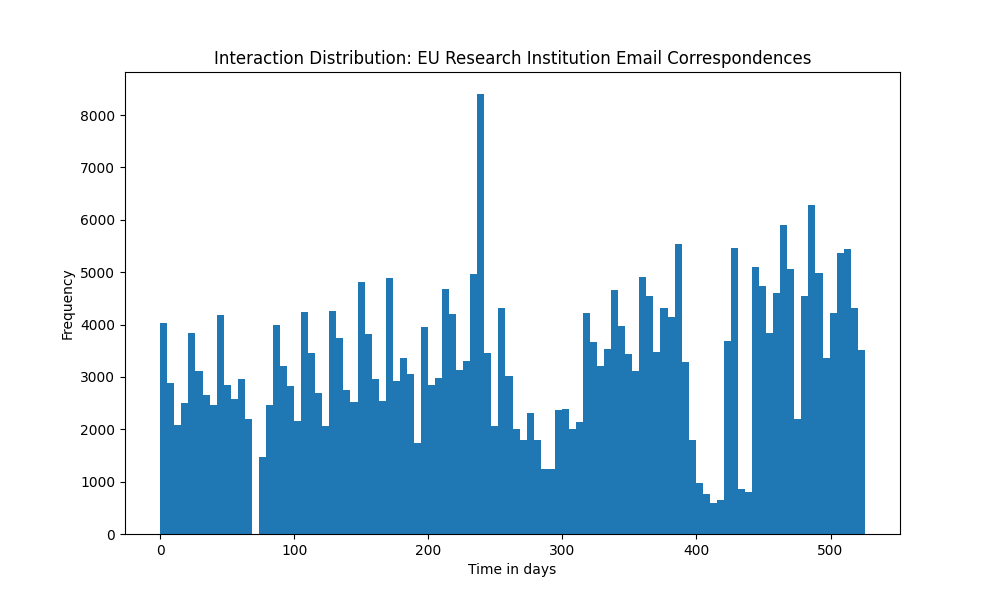
\includegraphics[width=\textwidth]{0_images/reallife_dataset_2_dist.png}
    \caption{Distribution of Real Dataset 2: EU Emails}
    \label{fig:RLdataset2}
\end{figure}


\subsubsection{Real Dataset 3: Student interactions in Lyon Primary School}
\label{sec:Data:RealData:RealDataset3}
Dataset can be found here: \href{http://www.sociopatterns.org/datasets/co-location-data-for-several-sociopatterns-data-sets/}{http://www.sociopatterns.org/datasets/co-location-data-for-several-sociopatterns-data-sets/}
\\\\
The third real-life dataset consists of co-location data of the students and teachers of a primary school in Lyon, France.
The original dataset consists of 241 individuals with 6.594.492, 20-second co-locations, meaning face-to-face interactions that persist over the span of 20 seconds.
The first interactions happening at $t_{min} = 34,240$ seconds and the last at 151.960 seconds.
The data is essentially split in two, temporally, and around half of interactions, 3.510.605, happen before time $t_{max} = 65,840$ seconds.
The dataset used for the project is this first half, consisting of $N = 237$ nodes with $n = 3,510,605$ interactions.
%From this half, the $n = 958,220$ interactions of 98 students and teachers are utilized.

The timestamps are transformed to hours, starting at hour 0 and ending at 84.25, by the following formula:

\begin{equation}
    t_i = \left(\frac{t_{max} - t_{min}}{3 \cdot 60} \right) \cdot \frac{t_i - t_{min}}{t_{max}}
\end{equation}
The distribution of these interaction have the distribution shown in figure \ref{fig:RLdataset3} below:

\begin{figure}[H]
    \centering
    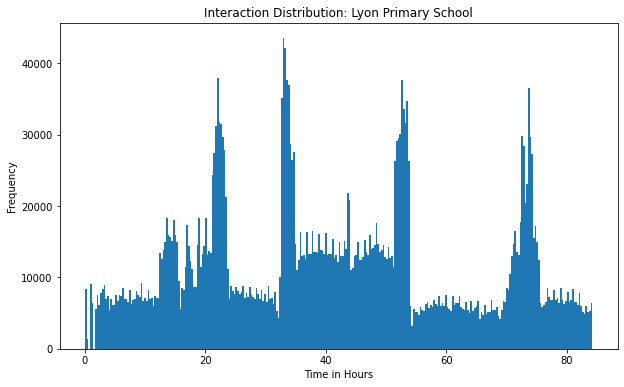
\includegraphics[width=\textwidth]{0_images/real_dataset_3_dist.png}
    \caption{Distribution of Real Life Dataset 3: Lyon Primary School}
    \label{fig:RLdataset3}
\end{figure}







